\chapter{Implementation process}
\label{chap:impl}

\section{Components of Genode network stack}

\begin{figure}
    \centering
    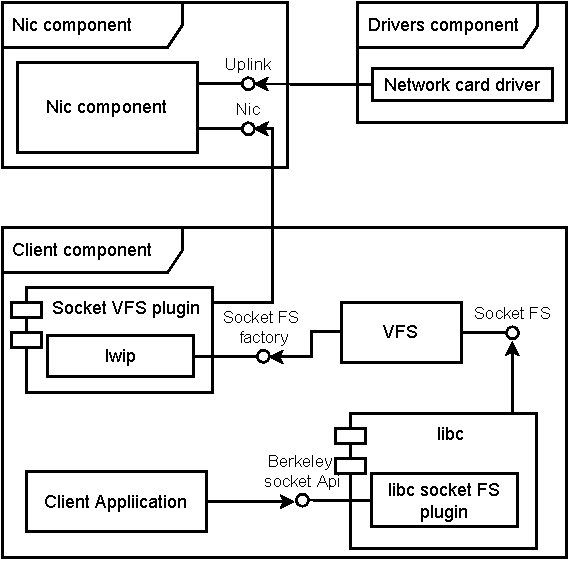
\includegraphics[]{figs/genode-network-stack.pdf}
    \caption{Components of Genode network stack}
    \label{fig:net-components}
\end{figure}

Before discussing the implementation details of developed persistent TCP stack
it is necessary to consider how Genode network stack works. Fig.
\ref{fig:net-components} depicts components and libraries that are required to
enable network access for a client application. In this diagram the Nic acronym
stands for Network interface controller. Nic component is a mediator for
packets that are produced and consumed by applications and network drivers.  As
can be seen from the diagram, Nic interface provides two RCP interfaces: the
Uplink interface is used by network drivers, and the Nic interface is used by
client applications. Nic interface exposes network packets as Ethernet frames.

The Nic RPC interface is almost never used directly. Instead most applications
tend to use the Berkeley sockets API, which include well-known functions
socket(), bind(), connect(), listen, and others. This API is provided by libc.
Genode's libc is based by the FreeBSD libc and its functions are implemented by
so-called libc plugins. Berkeley sockets API is implemented in the libc socket
FS plugin. This plugin depends on Genode VFS. The plugin expects VFS to expose
each socket as a set of virtual files.

The libc socket FS plugin should be used in conjunction with a socket VFS
plugin. Such a VFS plugin generally is merely an adapter between a Nic session
and port of some popular TCP stack. The actual TCP stack implementation is
denoted by "lwip" on Fig. \ref{fig:net-components}. For now, two TCP ports
are available in Genode -- lxip, which is a port of Linux TCP/IP stack, and
lwip. Usually TCP stack is statically linked within a VFS plugin, and VFS
plugin is a shared library that exposes a single symbol: function to
instantiate a VFS plugin.

Each Genode component has an initial configuration that is written as an XML
"config" node. The node also may contain configuration for VFS, if a component
needs one. Configurations for VFS and libc are located at "vfs" and "libc"
sub-nodes of "config". Each VFS directory can have a plugin that will handle
access to the directory and all its subdirectories and files. Plugin libraries
are resolved in the runtime when a component initializes. To use libc with a
socket VFS plugin component should place a VFS plugin to some directory and
pass a path to this directory to the libc config. A minimal example
configuration for Genode component that is able to use network is given in the
Appendix \ref{appex:conf-sample}

I had a hypothesis that a persistent TCP stack can be implemented as a VFS
plugin wrapping another VFS plugin. The inner VFS plugin would provide a "real" 
TCP interface, and the outer plugin would manage the inner one to save and
restore its state as needed. I decided to name the plugin PTCP for "persistent
TCP". PTCP can use any VFS plugin that provides TCP sockets as set of files. At
the runtime PTCP loads shared library with an inner plugin. This dynamic
linkage was done by design, with the assumption that system that has components
using PTCP can also have components that use plain lwip VFS plugin, since it is
popular among Genode software.

\section{Snapshot structure}

The PoG port was not ready during the most of the time this work was in
progress. However, the technique this port uses to achieve persistence was
known in advance. The technique is snapshotting just like in plain Phantom OS.
To use snapshotting I needed to decide what data should be included in a
snapshot. I tried several different approaches with respect to the snapshot
content. The content of a snapshot is discussed in detail in this section.

\subsection{Access to TCP internal data structures}

The first attempt to snapshot a TCP implementation concluded in saving the
state of socket state machine. This is the second approach proposed in Section
\ref{sec:meth:fsms}. For simplicity I decided to start with saving and
restoring a specific VFS plugin -- lwip. lwip represents each socket as a
protocol control block (PCB). PCB is a structure that holds values that are
required for protocol functioning. For example, TCP PCB encapsulates current
connection state, SEQ number, ACK number, and several other fields. lwip keeps
all PCBs in the few linked lists. References to these lists are located at
static section of lwip binary.

The challenge was to access the lists from the PTCP plugin. Indeed, PTCP could
access the address space of the inner plugin but the problem was that lwip is
statically linked to the vfs\_lwip plugin. Moreover, all lwip symbols are
erased from the binary at the linkage time. The only symbol exposed from
vfs\_lwip is a function that returns a factory for lwip plugin instances. To
overcome this issue I reconfigured vfs\_lwip to include lwip as a shared
library. With this reconfiguration I was able to access lwip internal
structures from PTCP plugin. Both vfs\_lwip and PTCP used the lwip shared
library. The VFS pluigins existed in the same Genode component, so they used
the same "instance" of lwip. Relationships between the libraries at that point
of time are presented at the Fig. \ref{fig:lib_deps}. There lwip\_dl.lib.so
denotes lwip in form of shared library.

\begin{figure}
    \centering
    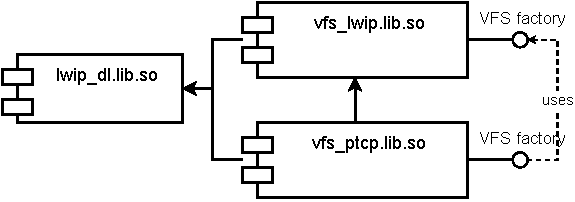
\includegraphics[]{figs/ptcp_libs.pdf}
    \caption{Relationships between the libraries comprising PTCP}
    \label{fig:lib_deps}
\end{figure}

After I manage to access the internal state of lwip in form of PCBs I started
implementing saving it to persistent storage. A PCB is a C structure and I
tried to save each PCB corresponding to socket field by field to a file.
However, in the process of implementing I discovered the two issues that made
me abandon this approach. The first problem that I discovered was a rather
complex structure of the PCBs. The tcp\_pcb structure includes more than 60
members and some of them are not atomic values but either nested structures or
buffers. Also list of members of tcp\_pcb can vary depending on compile-time
config. However, I could easily solve this issue by treating each structure as
a byte array and copy it to the snapshot file and back to memory as needed. The
second and the main issue was that despite my assumption sockets state was
stored not solely on lwip PCB lists but also at the lwip VFS plugin level and
even in libc socket plugin. Therefore even if I would proceed with snapshotting
lwip internal structures I would not achieve desired effect. The approach with
saving internal structures of TCP stack also is not universal. It should be
adapted to each new TCP stack implementation.

To mitigate the two issues above I decided to abandon the idea of saving state
holding structures on the field-by-filed basis and instead proceed with
snapshotting virtual memory spaces of all components of Genode network stack
located within the client component. This include VFS plugins and part of libc
responsible for sockets API.

\subsection{Approach with memory}
As a second approach I tried to save memory pages that belong to network stack
and restore them on component startup. Genode manages virtual memory with use
of Allocator class instances. I have subclassed the base Allocator class and
created a class that was able to track virtual addresses it allocated, save
allocated regions to a file, and load them back to virtual memory. I applied
this allocator so that it saved and restored heap dataspaces related to libc,
lwip VFS plugin and lwip itself.

At this point I faced a problem related to restoration of heap space. If a heap
space is prepopuilated before an allocator is passed to its user it will never
use this space. The allocator will never return adresses belonging to the
address range of the space in response to the user's allocation request. After
I understood the problem I changed the implementation so that it overwrote an
address range \textit{after} it was returned in response to user's request.
That is, the program detected that the TCP stack finished its initialization
and then overwrote its address space with memory from previous boot of the
system. However, this approach did not work properly by the two reasons. 

The first reason was the presence of the kernel capabilities inside the address
space. Capabilities are used throughout almost each part of the Genode OS
framework. In fact, the component can not exist without using at least one
capability, and can not execute any code without using at least three - namely
Parent, CPU and RAM capabilities. lwip VFS plugin should use eight more
capabilities to use Nic RPC interface. Each allocated address range consumes
one dataspace capability to use virtual memory service RPC interface. This
ubiquity of capabilities and the fact that they become invalid after restart
make straightforward saving and loading of component's memory to disk
impossible. This approach becomes even more complicated if a snapshotted
component uses shared memory, which is the case for Nic interface clients. Nic
servers use zero-copy packet delivery mechanism to increase memory throughput.
This mechanism implies establishment of shared memory between client and server
components. For example, a memory address range might be shared with other
components that are not persisted. In this case the persistent component
expects its sibling to use the same memory space they used for memory-mapped
communication earlier, and the sibling is unaware of any communications before
power loss.

The second and the main issue with the raw memory saving approach is that
layout of structures in the memory is undefined. The layout depends on order
of allocation requests and presence of Address space layout randomization
(ASLR). The interface of Allocator class does not allow the allocator determine
the purpose of allocation, i.e. what structure will be placed in the newly
created dataspase. These two issues explain why I decided to stop work in this
direction and decided to shift focus to a completely different approach.

\subsection{Observer for TCP state machine}

The main idea of the new approach was to build a tracker that will know the
internal state of every socket without directly accessing those states. This
idea uses the third approach that was proposed in section \ref{sec:meth:fsms}. 
We can treat each socket as a graybox where the inputs are user-called
functions and TCP segments from network. The outputs of this box are packets
that are scheduled for sending at the Nic server and data chunks delivered to
clients of TCP stack.

The libc transforms user calls to Berkeley socket API into file access
operations. This operations are processed by Genode VFS. The VFS delegates all
operations to its plugins, and when a plugin is not found, an error is thrown.
In my case all socket operations were processed by the PTCP plugin. To track
user calls I created a wrapper around FS factory exposed by the PTCP inner
plugin. This wrapper creates a new proxy filesystem that delegates processing
all calls to FS returned by the inner plugin. The proxy FS is equipped with a
tracking delegate that notifies the tracker about each accessed file.

The tracker is a class that is responsible for registering new sockets and
storing socket metadata. The tracker keeps a one structure with metadata per
each socket. When the tracking delegate notifies the tracker it searches the
socket metadata that corresponds to the accesses file. Then the tracker
updates the structure according to the new socket state. The tracker also keeps
in account the result of file access. For example, when writing to a bind file
finished with error, the state of a socket does not change. Hence, no need to
update the correspondent metadata structure.

Certain parts of socket state required for proper setup of the connection are
not exposed to a VFS plugin by a TCP stack. These parts include sequence and
acknowledgement numbers. To enable tracking and control for the arriving
network packets I added a secondary Nic server that scans headers of incoming
packets and keeps a metadata record with Nic-specific data for each noticed TCP
connection. At the snapshot time PTCP queries the proxy to obtain these records
if they are needed. The presence of tracker allows PTCP to intercept incoming
packets without changing code of the inner plugin. 

To restore state of the sockets I added a client library that is used on
component startup. During the initialization the library reads a snapshot,
reopens each socket present in the snapshot, and brings them to the last known
state. Restoration of the state is performed with the sequence of calls to
Berkeley socket API, and RPC calls to the proxy Nic server. The proxy Nic is
responsible for restoration of those parts of socket state that can not be set
by user. For example, these parts include sequence and acknowledgements
numbers. 

To restore acknowledgement numbers for sockets that were created by accept()
call I save the original segment that initiated segment and the third, ACK,
segment in the TCP handshake. At restoration time I restore parent socket for
the accepted one. It should always exist because any accepted socket arise from
sequence of listen() and accept() calls. And to use listen() call there should
exist a listening socket. After the parent socket is restored, I issue the
accept() call and emulate an incoming connection request. The request is
emulated with the help of the custom Nic server discussed above. It sends a SYN
segment to the TCP stack on local host. The sequence number in this segment is
modified to match the last acknowledged byte at snapshot moment.

To restore values of sequence numbers the Nic proxy acts similar to the NAT
mechanism in routers. But instead of changing source and destination ports
values in TCP headers the Nic proxy changes sequence numbers for outcoming
segments headers so that the remote side of the connection would recognise the
newly opened socket as the old one. It also changes ACK number for incoming
segments before they are delivered to TCP stack. To keep the segment valid from
TCP point of view Nic incrementallly updates TCP checksum after modification. 

The idea of proxy was highly inspired by the use of Linux kernel packet filters
in \cite{rocks_racks}. The complete architecture of network stack with tracking
and restoring of TCP sockets states is presented on Fig.
\ref{fig:track_components}.

\begin{figure}
    \centering
    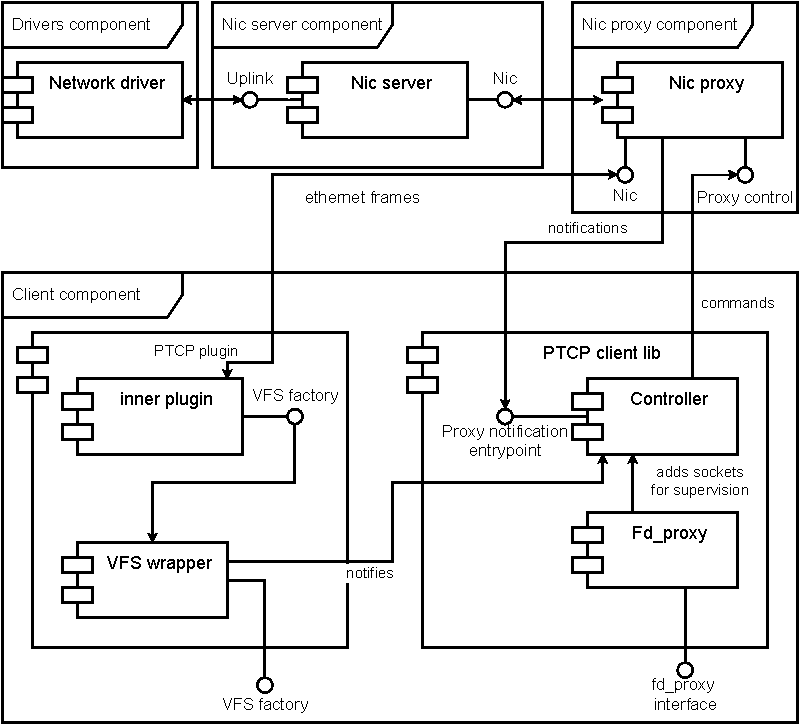
\includegraphics[]{figs/tracking_tcp_stack.pdf}
    \caption{Structure of software components involved in snapshotting of TCP stack}
    \label{fig:track_components}
\end{figure}

\section{Sockets naming}

To use sockets an application should have a way of distinguishing between them.
An application in a persistent environment expects that it will be able to use
objects using the same identifiers before and after restart. This explains a
need in a persistent socket handles for PTCP.

Each new socket created with the Berkeley socket API has a unique identifier.
This identifier is an integer number that corresponds to a socket file
descriptor. In Genode these file descriptors are stored inside the libc. They
are assigned to the files in the order of opening in a sequential manner.
Neither libc no Berkeley sockets API have a way of expressing desired file
descriptor when a socket is opened. That is why it is impossible to guarantee
that sockets will have the same libc file descriptors before and after restart.

To workaround this problem I created a proxying file descriptor mechanism. This
mechanism is merely a map between a persistent file descriptor and a libc one.
The persistent handles are saved together with socket metadata blocks used in a
restoration phase. This allows to restore state of each socket and prepopulate
the map with new libc file descriptors before returning control to an
application. The drawback of this approach is that applications can not use
Berkeley socket API with the persistent socket descriptors until the proxying
mechanism is not integrated to the libc. 

This mechanism cannot exist within the VFS plugin, so I moved it into a client
library. Mechanism cannot exist there because it is not desirable for
application to be linked with a VFS plugin and it is not guaranteed that VFS
will bind to already loaded VFS plugin instead of loading a new one. As it was
impossible to get rid of the client library, I decided to move controller
inside the client library. The benefit of that move was easier development,
since I was able to use libc inside the client library. VFS plugins, on the
other hand, generally unable to use it. The controller and the proxying mechanism
denoted at the Fig \ref{fig:track_components} as "Controller" and "Fd\_proxy"
correspondingly.

\section{Snapshot consistency}

Saving state of a TCP stack to persistent memory is not an atomic operation. It
is not desirable to stop execution of the entire component until it is
finished. That is why forming of snapshot structure and writing to a file is
executed in a separate thread. However, this creates a problem of making a
snapshot consistent. For example, while a socket metadata structure is being
written to persistent storage the socket might receive a packet. The controller
will intercept the packet and change the metadata structure accordingly. This
modification would make the structure corrupted. 

To avoid this problem I created a critical section inside a snapshotting
function. When execution flow enters this section, it acquires the mutex that
blocks all calls to PTCP VFS plugin and suspends the Nic proxy. The function
suspends the Nic proxy via the Proxy control RPC interface. The Nic proxy 
handles RPC requests and incoming packets in the different threads. That allows
to suspend packet receiving thread until snapshot structure will be formed.
When the process of forming is complete, PTCP calls an RPC method that resumes
execution of the packet processing thread in the Nic proxy. Then it releases
the PTCP VFS plugin mutex. 

The incoming packets that arrived while Nic proxy was suspended are buffered by
a Nic server component. To avoid overflow of the buffer I tried to make
critical section as short as possible. Due to this the writing of memory to the
disk is not within the critical section. Instead, the critical section contains
only copying values that will be written to a thread-local storage. This
storage is used solely by the snapshot thread and thus is not modified
concurrently. After snapshot is formed it is safely written to the persistent
memory file. For now this persistent memory is just a file, but in principle it
can be anything, even a part of Phantom OS snapshot.

\section{Integration with Phantom OS}

The goal of this paper is to design a persistent networking stack suitable for
Phantom OS. Due to this, it is possible to include a snapshot of the TCP stack
into the Phantom VM snapshot structure. However, I decided that a persistent
network stack can be useful not only for the Phantom OS but also for other
persistent systems. These systems be implemented entirely in Genode and can use
other mechanisms for persistence. Due to this, I decided to make an abstract
interface that has functions for saving and loading binary data from persistent
memory.

For simplicity, the only implementation of this service saves its state
directly to the hard drive volume attached to VM. An implementation that saves
and loads data using the Phantom snapshotting mechanism is currently in
progress.

Phantom OS should notify PTCP about snapshot so that their shapshots would be
synchronized. The component that hosts Phantom VM implements Snapshot\_notifier
RPC interface. This interface allows an application to suscribe to snapshot
notifications. When PoG begins a snapshot the application receives the
notification and starts snapshot process of itself. After the snapshot of PTCP
is finished it is ready to process new packets. Restoration of the PTCP state
is performed when its component initializes.

The duration of PTCP snapshot is generally shorter than one of the PoG port.
This might create issues with snapshot consistency. However, it is hard to
reason about this issue since PTCP was not tested together with PoG port.
